% Rebuilt against the official 2027 IEEE Aerospace class.
\documentclass[twocolumn,letterpaper]{IEEEAerospaceCLS}
\usepackage{amsmath,amssymb,graphicx,booktabs,array}
\usepackage[T1]{fontenc}
\usepackage[hyphens]{url}
\usepackage[hidelinks]{hyperref}
\usepackage{microtype,placeins}
\geometry{top=0.75in,bottom=0.75in}
\urlstyle{same}
\newcolumntype{L}[1]{>{\raggedright\arraybackslash}p{#1}}
\newcommand{\gate}[1]{\textsc{#1}}
\renewcommand{\arraystretch}{1.12}
\begin{document}
\title{System Architecture and Service Envelope of a Multirotor Communications Relay}
\author{Noah Stephenson\\United States Military Academy\\West Point, NY 10996\\noah.stephenson@westpoint.edu
\thanks{U.S. Government work not protected by U.S. copyright}}
\maketitle
\thispagestyle{plain}\pagestyle{plain}
\begin{abstract}
A communications relay can clear an obstructed path while imposing an aircraft demand that a small multirotor cannot sustain. This paper develops a reproducible architecture case study that separates these two questions: whether an outbound relay path has sufficient received-level margin, and whether its carrier can support the payload for the required stationary dwell. The architecture assigns mission traffic to a black-box radio payload and assigns positioning, electrical support, and mechanical retention to the carrier. A geometric visibility test and free-space link budget define the communications screen. A constant-disk-loading hover model then closes the battery, propulsion, and structural mass balance on energy-sized and power-sized battery branches. Its aggregate hover coefficient is fitted to five published NASA test points. Comparisons with three commercial quadrotors excluded from that fit give hover-time differences from -6.7 to +3.2 percent under the stated manufacturer conditions and an assumed 25 W auxiliary load; these comparisons do not validate the proposed relay aircraft or its structural model. For the declared 0.20 kg, 14 W payload, the reference link-margin boundary is 25.0 km of endpoint separation at a midpoint relay height of 120 m. A deterministic 12 dB excess-loss case reduces that boundary to 6.3 km. The reference carrier, which carries no operating-condition margin beyond the laboratory hover calibration, reaches its exploratory rotor-size limit at 42.1 minutes and has no finite mass closure at or above 52.4 minutes, within this model. The scatter of the individual calibration points alone moves the first boundary between 33 and 49 minutes. At a fixed 10 km separation, 30 minutes closes at 4.77 kg, 45 minutes closes at 15.15 kg outside the physical screen, and 60 minutes has no finite solution. Of 90 baseline grid cases, 18 pass both screens; 6 have excessive finite size, 6 have no closure, and 60 fail connectivity. The case study shows how identifying the limiting mechanism supports early architecture decisions. Its results describe conditional outbound hover service, with full-mission energy, packet performance, and physical verification left unresolved.
\end{abstract}
\tableofcontents
%======================================================================
\section{Introduction}
%======================================================================

A relay aircraft changes the geometry of a communications problem. A ground station may be unable to reach a remote aircraft because an obstruction crosses the direct path. Placing a radio above the obstruction can provide two clear paths, one to each endpoint. Research on unmanned aircraft systems (UAS) has examined this opportunity through aerial networking and mobile relaying \cite{zengmag}, \cite{tutorial}, \cite{zengrelay}. The aircraft must sustain the useful geometry while carrying and powering the radio. This makes the communications requirement an aircraft resource requirement as well.

Consider a 10 km separation, a remote aircraft at 100 m, and an 80 m screen between the endpoints. A midpoint relay at 120 m clears the screen in the declared geometry. Whether it can remain there for 30, 45, or 60 minutes depends on a different calculation. More battery adds mass, greater mass requires more hover power, and that power requires additional battery. A consistent mass balance can lie within a small-aircraft envelope, lie outside it, or have no finite solution under the assumed scaling relations.

This paper follows that example from system responsibilities through link margin and carrier sizing to a combined service screen. Section 2 defines the architecture and assessed interval. Section 3 states the models and evidence supporting their coefficients. Section 4 presents the worked case and sampled envelope, and Sections 5 and 6 explain the decisions and limitations. An appendix gives the complete mass balance for reproduction.

\subsection{Related Work and Contribution}

Communication and aircraft sizing research already supplies the pieces used here. Zeng, Zhang, and Lim optimized relay transmit power together with relay trajectory \cite{zengrelay}. Zeng, Xu, and Zhang combined rotary-wing propulsion energy with communication energy under throughput constraints \cite{zengenergy}. Yan et al.\ treated battery weight as a design variable that trades stored energy against the power needed to lift it \cite{yan}. Rodrigues et al.\ placed relay positioning inside a propulsion-aware energy model \cite{rodrigues}. On the aircraft side, Russell, Theodore, and Sekula built conceptual sizing models for small quadcopters from test data \cite{russell2018}. They reported that their sizing did not close for hover missions beyond a certain length. Bershadsky, Haviland, and Johnson matched motors, propellers, and batteries to mission requirements \cite{bershadsky}. Table~\ref{tab:prior} places these alongside the present study.

The contribution is an explicit, reproducible assessment of one relay architecture. Payload mass and electrical demand connect the carrier calculation to fixed radio assumptions; the resulting screens identify connectivity failure, excessive finite size, and mathematical nonclosure separately. The analysis includes an aggregate hover-power fit and comparisons with published commercial hover times to examine part of the carrier model. It offers a worked engineering case, with traceable assumptions and distinguishable failure mechanisms, rather than a new optimization method or a claim of superiority over the cited approaches.

The research question is narrow. Under the declared service and aircraft assumptions, how far apart can the endpoints be and how long can the relay stay on station before one of the two checks fails? The quantitative work covers stationary one-way service. It does not establish delivered throughput, full mission energy, or measured flight performance.

\begin{table}[!tb]
\caption{Related work and its relationship to this study}
\label{tab:prior}
\centering\small
\begin{tabular}{@{}L{0.8in}L{1.0in}L{1.05in}@{}}
\toprule
Reference & Emphasis & Relationship \\
\midrule
Zeng et al., 2016 \cite{zengrelay} & Relay power and trajectory optimization & Relay placement and power design is prior work \\
Zeng et al., 2019 \cite{zengenergy} & Propulsion and communication energy together & Combined energy reasoning is prior work \\
Yan et al., 2021 \cite{yan} & Battery weight and available energy & Battery mass tradeoffs are prior work \\
Rodrigues et al., 2022 \cite{rodrigues} & Propulsion-aware relay positioning & Relay endurance and service are prior work \\
Russell et al., 2018 \cite{russell2018} & Small quadcopter sizing from test data & Sizing feedback and failure to close are prior work \\
Present study & Architecture screening with a hover-power fit & Conditional envelope with explicit failure mechanisms \\
\bottomrule
\end{tabular}

\vspace{2pt}
\begin{minipage}{\columnwidth}\footnotesize
These are the closest conceptual precedents, not a complete survey. This study claims no methodological advantage over them.
\end{minipage}
\end{table}

%======================================================================
\section{System and Assessment Boundary}\label{sec:arch}
%======================================================================

The relay aircraft carries a communications payload and holds an assigned position. As Figure~\ref{fig:arch}(a) shows, a ground endpoint labeled G exchanges traffic with a remote aircraft labeled U, and the payload passes that traffic between them. The payload is treated as a black box. This means it is described only by what it demands from the aircraft: 0.20 kg of mass, 14 W of direct current (DC) power, and a fixed radio frequency (RF) output. The aircraft supplies the airframe, propulsion, battery and power distribution, avionics, the command radio, and the payload mount. Operators, ground equipment, the remote aircraft, and spectrum authorities stay outside this boundary.

Two design commitments follow from that split. The aircraft-to-payload boundary carries only regulated power and mechanical retention, which defines the intended accommodation boundary. Similar mass and power alone do not establish interchangeability; mounting, voltage, thermal behavior, and electromagnetic compatibility would also need verification. The operator commands the aircraft on a separate radio path, as an architectural allocation distinct from the mission traffic. While this separation is deliberate, it is an allocation of responsibility and not a demonstrated fault isolation, since both paths still share one battery and one airframe.

Only the time on station is assessed quantitatively. A full mission would run from preparation through launch, transit, establishing position, relaying, monitoring, and recovery. This paper calculates the relay interval alone, and only in the direction from G through the relay R to U. The battery reserve holds energy back from that interval, but it is not a transit or recovery calculation.

\begin{figure*}[!tb]
\centering
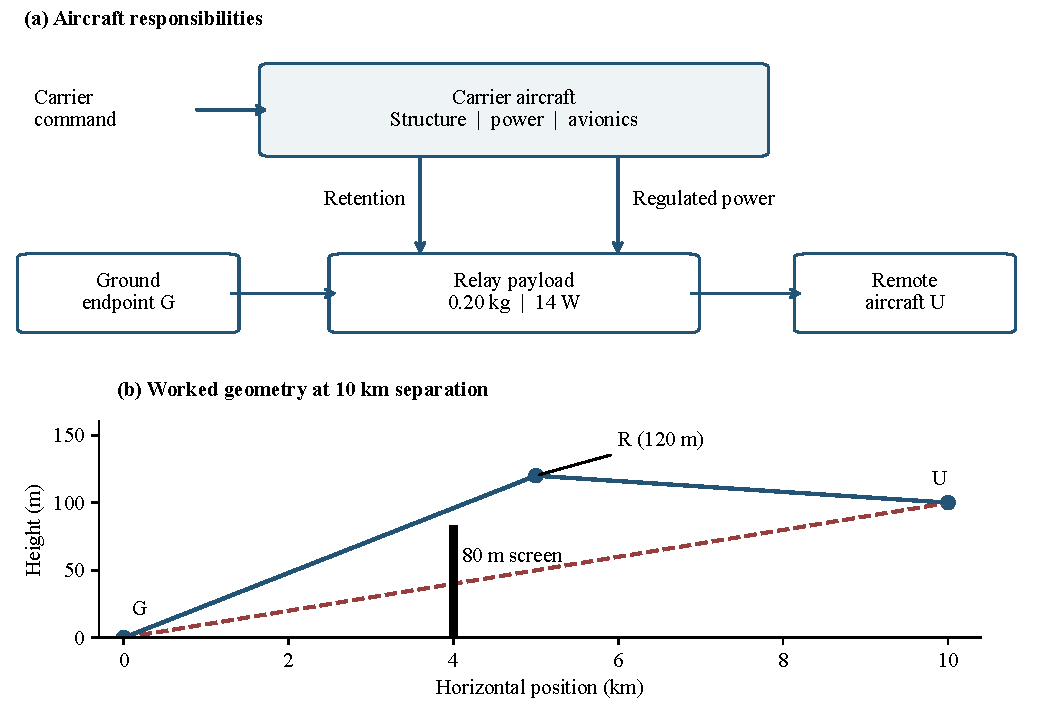
\includegraphics[width=\textwidth]{figs/fig1_architecture_geometry.pdf}
\caption{Relay architecture and the worked geometry. (a) The aircraft supports a black-box payload across two connections, mechanical retention and regulated power, and the operator commands the aircraft on a separate radio path. (b) At 10 km separation the ideal screen blocks the direct path and clears the relay path. The screen is a declared scenario, not measured terrain, and the command separation is an allocation, not a demonstrated fault isolation.}
\label{fig:arch}
\end{figure*}

%======================================================================
\section{Method}\label{sec:methods}
%======================================================================

\subsection{Declared Inputs}

\begin{table}[!tb]
\caption{Declared inputs and calibrated coefficients}
\label{tab:inputs}
\centering\small
\begin{tabular}{@{}L{1.15in}L{0.85in}L{0.85in}@{}}
\toprule
Quantity & Value & Status \\
\midrule
Endpoint separation & 5, 10, 20, 30, 40, 60 km & Declared grid \\
Dwell & 10, 20, 30, 45, 60 min & Declared grid \\
Ground, remote height & 0, 100 m & Common datum \\
Relay position; height & midpoint; 60, 120, 240 m & Not optimized \\
Screen height; position & 80 m; 0.40 of span & Declared scenario \\
Frequency; bandwidth & 2400 MHz; 5 MHz & Bandwidth unused \\
Transmit levels & 30 dBm ground; 32.04 dBm relay & Declared \\
Antenna gains & 6 dBi endpoint; 2 dBi relay & Declared \\
Other loss; threshold & 6 dB; $-90$~dBm & Declared \\
Extra loss & 0 dB; 12 dB case & Declared scenario \\
Payload mass; DC power & 0.20 kg; 14 W & Device data plus allowance \\
\midrule
Effective $FM$ parameter & 0.6203 & Aggregate fit \cite{nasatm} \\
Structure intercept & 0.163 kg & Anchored to sized design \cite{russell2018} \\
Battery specific energy $e$ & 192.1 Wh/kg & Production pack \cite{djim30} \\
Drive efficiency $\eta$ & 0.83 & Declared \\
Disk loading $DL$ & 60 N/m$^2$ & Declared \\
Condition multiplier $k_{env}$ & 1.15 & Declared; absorbed by fit \\
Battery specific power $p$ & 900 W/kg & Declared \\
Usable fraction $u$ & 0.72 & Mission policy \\
Thrust margin & 1.75 & Declared \\
Fixed carried mass $F$ & 1.116 kg & Declared allowances \\
Structure growth fraction & 0.18 & Declared \\
Size limits & 15 kg; 0.75 m rotor & Screening limits \\
\bottomrule
\end{tabular}

\vspace{2pt}
\begin{minipage}{\columnwidth}\footnotesize
Declared values are analysis assumptions rather than approved requirements. The aggregate hover fit, structural anchor, and battery reference are explained below; the appendix gives all mass-model coefficients. The size limits screen results; they are not owner requirements.
\end{minipage}
\end{table}

The study samples declared geometries and durations rather than observed operations. Heights are measured from a common ground datum, with the ground endpoint at 0 m and the remote aircraft at 100 m. The relay sits at the horizontal midpoint at 60, 120, or 240 m. Endpoint separation takes six values from 5 to 60 km and dwell takes five values from 10 to 60 minutes. Table~\ref{tab:inputs} lists these inputs. The baseline scenario places an 80 m opaque screen at 40 percent of the separation. Four variants move that screen, one variant adds 12 dB of loss, and one comparator removes the screen entirely. These are stylized visibility cases, not terrain.

The payload values come from a commercial mesh radio module with a published mass of 102 g, 5 W receive consumption, 14 W peak consumption, and 1.6 W maximum transmit power \cite{doodle}. The model adds 98 g for unselected integration hardware and applies the 14 W peak value continuously. Applying the listed peak continuously is a sizing assumption. The stated maximum RF output and DC consumption have not been verified as a simultaneous operating point. The receiver threshold of $-90$~dBm is one common assumption applied to every receiver, and the 5 MHz bandwidth is recorded as context that never enters the margin calculation.

\subsection{Link Check}

The link check asks two questions about each path: is it clear, and is the received signal strong enough. A path is clear when the straight line between its endpoints passes above the screen. For a screen of height $H$ standing at a fraction $s$ of the separation, similar triangles give the relay height at which the first hop begins to clear,
\begin{equation}
h_{th}=z_G+\frac{(H-z_G)\,r}{s},
\end{equation}
where $z_G$ is the ground endpoint height and $r$ is the relay position as a fraction of the separation. At the baseline values of 80 m, $s=0.40$, and $r=0.5$, this threshold is 100 m. This means a relay at or below 100 m leaves the first hop blocked. Heights are compared strictly, so a path that just grazes the screen counts as blocked. This expression applies to a screen between the ground endpoint and the relay, as in every screened scenario here. The second hop does not cross that screen. The screen is an opaque plane, and the model includes no diffraction, Fresnel-zone clearance, or earth curvature.

For a clear path, free-space loss over a distance $d$ in kilometers at frequency $f$ in megahertz is
\begin{equation}
L=32.44+20\log_{10}f+20\log_{10}d,
\end{equation}
following the free-space transmission relation \cite{itu525}, \cite{friis}. The implementation retains 32.44 for the unit conversion; P.525 prints the rounded value 32.4. The link margin is the received level above the receiver threshold,
\begin{equation}
M=P_t+G_t+G_r-L-L_0-L_x-S,
\end{equation}
where $P_t$ is the transmit level in dBm, $G_t$ and $G_r$ are antenna gains in dBi, $L_0$ is a 6 dB miscellaneous loss allowance, $L_x$ is the scenario loss, and $S$ is the $-90$~dBm threshold. The ground endpoint transmits at 30 dBm and the relay transmits at 32.04 dBm, which is the 1.6 W maximum expressed in dBm. A relay path passes only when both hops are clear and both margins are at least 0 dB. The check covers signal level only, so it says nothing about interference, scheduling, or delivered data rate.

\subsection{Carrier Sizing}

The aircraft side of the assessment asks whether an aircraft of consistent mass can hover with the payload for the requested time. Rotor disk area is set by holding disk loading constant at 60 N/m$^2$, so area grows in proportion to mass. Momentum theory then gives ideal hover power, and dividing by the rotor figure of merit and the drive efficiency converts that to electrical power \cite{leishman}, \cite{ndarc}. The result is proportional to gross mass $m$,
\begin{equation}
P=k\,m,\qquad k=\frac{g\,k_{env}}{FM\,\eta}\sqrt{\frac{DL}{2\rho}},
\end{equation}
where $FM$ is the figure of merit, $\eta$ the combined motor and controller efficiency, $DL$ the disk loading, $\rho$ the air density, and $k_{env}$ an assumed multiplier for operating conditions. Because this multiplier is held fixed during fitting, the fitted $FM$ absorbs it: the product $FM\,\eta/k_{env}$ is what the calibration identifies. The reference relation therefore reproduces the laboratory hover power and carries no net margin for operating conditions. At the calibrated values in Table~\ref{tab:inputs}, $k$ is 108.4 W/kg. The model therefore describes a family of aircraft that are resized as mass grows, not one airframe carrying a bigger battery. Applying a separate 15 percent operating margin on top of the fitted relation would raise $k$ to 124.7 W/kg and move the carrier boundaries reported in Section~4 from 42.1 and 52.4 minutes to 35.7 and 44.5 minutes.

The battery must satisfy two separate demands, and the larger one governs. Over a dwell $t$ in hours, the aircraft draws $P$ for hover plus a fixed 40.2 W for avionics and the payload, and only the usable fraction $u$ of the pack is available. The pack must also deliver the peak current that a thrust margin of 1.75 implies, which is 2.32 times hover power, with a further 15 percent allowance. With specific energy $e$ in Wh/kg and specific power $p$ in W/kg,
\begin{equation}
m_{b}=\max\!\left(\frac{(km+P_0)\,t}{u\,e},\ \frac{1.15\,(1.75^{3/2}km+P_0)}{p}\right).
\end{equation}
The reserve is part of the mission policy rather than the calibration. Holding back 20 percent after a 90 percent depth of discharge leaves $u=0.72$.

Adding the remaining masses closes the loop. Propulsion mass scales with peak power and rotor area, and structure carries a base mass plus a fraction of everything it supports. The payload, avionics, power electronics, and mount contribute $F=1.116$ kg. The appendix defines each component allowance. On each battery branch $j$, the terms are constant or proportional to $m$, so the implied mass is
\begin{equation}
m_{new,j}=a_jm+b_j.
\end{equation}
Here $b_j$ collects fixed masses in kilograms and $a_j$ is the branch growth factor, which is the fraction of any added kilogram that the aircraft must add again as battery, propulsion, and structure. Table~\ref{tab:inputs} gives the inputs behind both. The energy branch grows with dwell. The power branch remains unchanged. The physical mass map takes the larger battery requirement at each trial mass.

\subsection{When the Aircraft Closes}

A consistent sizing result is a fixed point: the mass implied by the resource calculation equals the trial gross mass. Each branch gives a candidate
\begin{equation}
m_j^*=\frac{b_j}{1-a_j}.
\end{equation}
For the positive intercepts and nonnegative coefficients used here, a candidate must have $a_j<1$, positive mass, and a battery requirement at least as large as the other branch at that mass. The appendix states these tests explicitly. A finite candidate on the wrong branch is not a solution.

The denominator explains why a longer dwell can have a disproportionate mass penalty. As the governing slope approaches one, a small increase in demand produces a large increase in closed mass. Once the energy slope reaches one, its positive intercept prevents a finite positive fixed point. This is a property of the assumed model; it is not a universal endurance limit for multirotors.

The power-branch slope is 0.5701 at the reference inputs. It governs the 10- and 20-minute examples, while energy governs the 30- and 45-minute examples. The implementation also applies relaxed iteration as a diagnostic, starting at 5 kg with a 200-iteration limit. The analytical branch test controls all reported physical quantities, so a timeout or the 50 kg iteration guard cannot be mistaken for physical nonclosure.

\subsection{Calibration and Check}

\begin{table*}[!tb]
\caption{Hover calibration and held-out endurance check}
\label{tab:calib}
\centering\small
\begin{tabular}{@{}L{1.55in}L{0.62in}r r r r r r@{}}
\toprule
Vehicle or test article & Role & Mass & Rotor dia. & Battery & Published & Model & Error \\
& & (kg) & (m) & (Wh) & & & \\
\midrule
3DR SOLO, NASA hover test \cite{nasatm} & fit & 1.51 & 0.254 & & 184.4 W & 180.7 W & $-2.0$\% \\
DJI Phantom 3, NASA hover test \cite{nasatm} & fit & 1.22 & 0.239 & & 172.1 W & 140.1 W & $-18.6$\% \\
3DR Iris+, NASA hover test \cite{nasatm} & fit & 1.28 & 0.244 & & 142.9 W & 146.6 W & $+2.6$\% \\
Drone America DAx8, NASA hover test \cite{nasatm} & fit & 5.59 & 0.279 & & 838.0 W & 827.5 W & $-1.3$\% \\
SUI Endurance, NASA hover test \cite{nasatm} & fit & 2.91 & 0.381 & & 281.5 W & 322.7 W & $+14.6$\% \\
DJI Matrice 30 \cite{djim30} & check & 3.77 & 0.406 & 263.2 & 36.0 min & 33.6 min & $-6.7$\% \\
DJI Matrice 4 \cite{djim4} & check & 1.22 & 0.274 & 99.5 & 42.0 min & 40.8 min & $-2.9$\% \\
DJI Mavic 3M \cite{djimavic} & check & 0.95 & 0.239 & 77.0 & 37.0 min & 38.2 min & $+3.2$\% \\
\bottomrule
\end{tabular}

\vspace{2pt}
\begin{minipage}{\textwidth}\footnotesize
Fit rows compare measured electrical hover power at the test article's own thrust and rotor size. Check rows were held out of the fit and compare published hover endurance at the manufacturer's stated discharge condition, which does not include the 20 percent mission reserve used elsewhere in this paper. The DAx8 and Endurance were hover-tested inside the wind-tunnel test section, where recirculation was not quantified; the other three NASA articles were tested in a laboratory about 30 ft from the nearest wall \cite{russell2016}. The DJI Matrice 350 was excluded because its published 55 minutes is forward flight at about 8 m/s rather than hover.
\end{minipage}
\end{table*}

The hover calibration estimates one aggregate coefficient from five NASA test points \cite{nasatm}. For each point, ideal induced power uses the measured supported thrust and that test article's total rotor disk area. Measured electrical power is voltage multiplied by the sum of motor currents. An unweighted least-squares fit through the origin gives $P_{\mathrm{elec}}=\gamma P_i$, with $1/\gamma=0.447676$. Holding drive efficiency at 0.83 and the environment multiplier at 1.15 gives an effective $FM$ parameter of 0.620274. The fit identifies their combined effect, not an independently measured rotor figure of merit. Its residuals range from $-18.6$ to $+14.6$ percent. Because the fit passes through the origin, each point's influence scales with the square of its ideal power, and the DAx8 carries 79 percent of that weight. Refitting to any single point moves the reference boundaries of Section~4 to between 33.0 and 49.2 minutes (rotor limit) and between 41.2 and 61.3 minutes (energy-slope crossing). The Phantom 3 and Endurance points, whose disk loadings of 67 and 63 N/m$^2$ are nearest the reference value, set both ends of that range. Other defensible estimators (mean ratio, geometric mean, quadrotors only) give 41.4 to 44.6 and 51.5 to 55.6 minutes. The two highest-leverage points were also the two tested inside the wind tunnel \cite{russell2016}. The fit treats the DAx8 as eight separate 11 in disks; the sources consulted do not state its rotor arrangement. If its rotors were coaxial pairs with four effective disks, the refit boundaries would rise to 58.8 and 73.5 minutes, although the implied DAx8 hover factor of 0.63 would then be well above that of the four quadrotors. Since interference between stacked rotors should lower that factor rather than raise it, this result argues for the eight-disk treatment used here.

The structural intercept is inferred separately from the NASA conceptual-design mass breakdown \cite{russell2018}. That breakdown describes a sized baseline design rather than a weighed vehicle: its 1.61 lb airframe comes from a fuselage weight trend plus motor-support and landing-gear fractions. The calculation reproduces its airframe allowance after subtracting the present model's structural growth and disk-area terms. Several carried masses in that subtraction are model allowances. The resulting 0.163173 kg is therefore conditional on those choices; it is not a directly measured empty-airframe mass or a separately validated structural law. The reference specific energy, 192.117 Wh/kg, comes from the published TB30 pack energy divided by its mass \cite{djim30}. That reference does not establish the assumed 900 W/kg continuous power capability for a selected relay battery. It is also the lowest pack value among the check aircraft. The Matrice 4 pack stores 99.5 Wh in 401 g, or 248 Wh/kg \cite{djim4}, and using that value moves the two carrier boundaries to 54.4 and 67.7 minutes.

Three commercial quadrotors are excluded from the five-point fit and used for a separate hover-time comparison \cite{djim30}, \cite{djim4}, \cite{djimavic}. Their own mass, rotor area, and nominal battery energy enter the calibrated power relation, with a common assumed 25 W auxiliary load. The calculation uses the published maximum-hover discharge condition without the relay mission's depth-of-discharge and reserve reductions. Differences range from $-6.7$ to $+3.2$ percent (Table~\ref{tab:calib}). The auxiliary allowance matters for the two smaller aircraft. With 0, 10, and 40 W instead of 25 W, the Matrice 30, Matrice 4, and Mavic 3M differences become $-1.5$, $+17.2$, and $+30.0$ percent; $-3.7$, $+8.2$, and $+17.8$ percent; and $-9.6$, $-11.9$, and $-8.2$ percent. Only the Matrice 30, whose hover power is large relative to the allowance, stays within 10 percent across that range. The two smaller aircraft are therefore consistent with the fitted relation rather than an independent test of it. The Matrice 350 figure is excluded because it describes forward flight. These comparisons provide a limited consistency check on hover power and energy accounting. They do not test the structural mass model, flight control, or a physical relay aircraft, and three published values do not establish a general prediction-error bound.

\begin{figure*}[!tb]
\centering
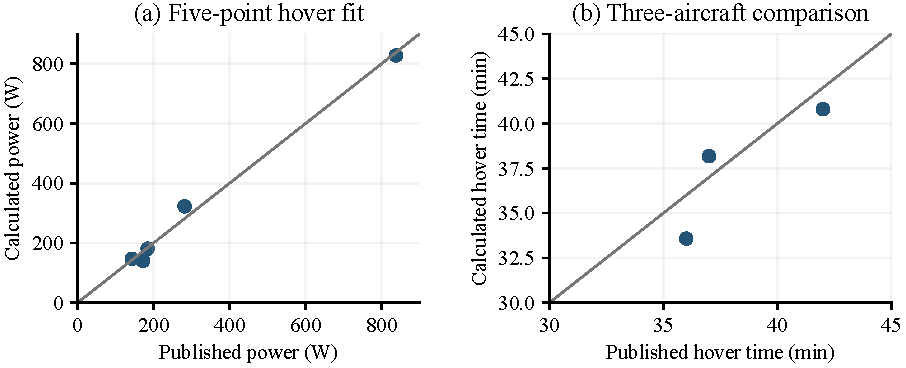
\includegraphics[width=\textwidth]{figs/fig2_calibration.pdf}
\caption{Hover evidence shown on separate axes. Left: measured and fitted electrical powers for the five NASA points. Right: published and calculated maximum-hover times for three aircraft excluded from the fit. A diagonal indicates agreement; neither panel validates carrier mass closure.}
\label{fig:calib}
\end{figure*}

\subsection{Size Limits and Decision Order}

A closed aircraft is screened against two size limits that keep the result in the small relay class. Gross mass must not exceed 15 kg, and the equivalent rotor diameter must not exceed 0.75 m, where the diameter comes from the total disk area $A=mg/DL$ shared across four rotors,
\begin{equation}
d=\sqrt{\frac{4A}{n\pi}}.
\end{equation}
At the reference disk loading the rotor limit binds first, since a 0.75 m rotor corresponds to a gross mass of 10.81 kg. A separate span check is twice the rotor diameter, so it repeats the rotor limit rather than adding a new one. These limits screen results. They are not approved requirements, and nothing in the analysis prevents a larger aircraft from existing.

Each case then receives one label from the first check that fails. If the direct path passes the assumed service screen, the case is \gate{direct}: relay benefit is not required by this criterion. Otherwise, if either relay hop is blocked or short of margin, the case is \gate{link fail}. Otherwise, if the aircraft has no solution, the case is \gate{no solution}, and if it has a solution outside the size limits, the case is \gate{too large}. What remains is a \gate{pass}, meaning a blocked or insufficient direct path, two passing outbound relay hops, and a finite carrier within the exploratory limits. Because connectivity is checked first, a \gate{link fail} label can hide an aircraft failure in the same case, so the case records keep both flags.

\subsection{Experiment and Verification}

Each scenario holds 90 cases, formed from six separations, five dwell values, and three relay altitudes. The primary payload is the 0.20 kg, 14 W case. Seven scenarios and three payload cases give 1,890 saved records, which are repetitions of the same grid rather than independent missions, so every count in this paper uses the 90-case denominator.

The repository carries 25 automated tests covering a hand-calculated hover case, the branch logic, the label order, the calibration script, and the two boundary calculations. A separate checker rebuilds every link from coordinates and solves the mass balance by bisection without using the production solver, then compares all saved records. All tests and checks pass at the commit cited in the Data Availability section. These confirm that the numbers follow from the stated equations. They do not confirm that a physical aircraft behaves this way.

%======================================================================
\begin{figure*}[!tb]
\centering
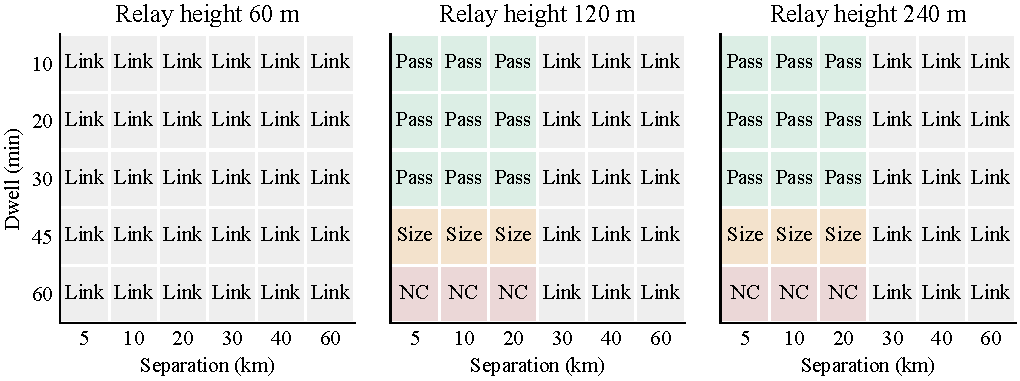
\includegraphics[width=\textwidth]{figs/fig3_service_map.pdf}
\caption{Baseline results for the 90 primary cases. \gate{pass} means the relay helps and the aircraft stays within the screening limits, \gate{size} marks a solution outside those limits, \gate{NC} marks a case with no solution, and \gate{link fail} marks the earlier link check. All cells in the 60 m panel fail visibility. Link failures in the 120 m and 240 m panels are clear but short of margin. No case in the baseline is direct-sufficient.}
\label{fig:map}
\end{figure*}

\section{Results}\label{sec:results}
%======================================================================

\subsection{Where the Envelope Ends}

For a midpoint relay at 120 m, solving the zero-margin condition gives a maximum endpoint separation of 25.0 km under the baseline RF assumptions. The ground-to-relay hop binds first. A 12 dB excess-loss allowance reduces that separation to 6.3 km. Both statements require a clear path. Dwell has no effect on this boundary because time does not enter the link model.

The reference carrier reaches the 0.75 m rotor limit at 42.1 minutes. At that point gross mass is 10.81 kg, so the rotor limit is tighter than the 15 kg mass ceiling. Finite closure persists until the energy-branch slope reaches one at 52.4 minutes. Thus the interval between these boundaries contains finite mathematical sizes that fail the physical screen. Figure~\ref{fig:closure} shows this transition without treating the divergent branch as a buildable aircraft.

The existing favorable and adverse parameter sets illustrate dependence on carrier assumptions. The favorable set gives a 126.9-minute physical boundary and a 157.0-minute energy-slope crossing. The adverse set has no physical pass even at zero dwell; its 6.4-minute energy-slope crossing is not an achievable service duration. These sets change several assumptions simultaneously. They are deterministic corners, not a confidence interval, and the reference is not a statistical midpoint.

\begin{figure}[!tb]
\centering
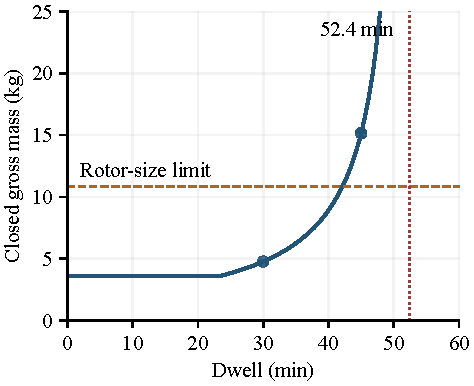
\includegraphics[width=\columnwidth]{figs/fig5_closure.pdf}
\caption{Reference carrier mass versus dwell, evaluated from the stated branch equations. The rotor screen binds at 42.1 minutes; the energy slope reaches one at 52.4 minutes. The plotted finite curve is clipped at 25 kg for readability.}
\label{fig:closure}
\end{figure}

\subsection{One Geometry, Three Outcomes}

\begin{table}[!tb]
\caption{Worked case at 10 km separation and 120 m relay altitude}
\label{tab:worked}
\centering\small
\setlength{\tabcolsep}{4pt}
\begin{tabular}{@{}r r r c r l@{}}
\toprule
Dwell & Mass & Rotor & Pack sized & Growth & Result \\
(min) & (kg) & (m) & by & factor $a$ & \\
\midrule
10 & 3.58 & 0.43 & power & 0.346 & \gate{pass} \\
20 & 3.58 & 0.43 & power & 0.500 & \gate{pass} \\
30 & 4.77 & 0.50 & energy & 0.654 & \gate{pass} \\
45 & 15.15 & 0.89 & energy & 0.885 & \gate{too large} \\
60 & none & none & none & 1.116 & \gate{no solution} \\
\bottomrule
\end{tabular}

\vspace{2pt}
\begin{minipage}{\columnwidth}\footnotesize
Link margins stay at 7.97 and 10.02 dB in every row, so the differences come entirely from the aircraft. The growth factor shown is the energy-limited one; the power-limited branch stays at 0.570 throughout. \gate{pass} means the relay helps and the aircraft stays within the screening limits, not that the design is validated.
\end{minipage}
\end{table}

The worked case fixes the geometry and varies only dwell, which isolates the aircraft behavior. At 10 km separation the screen stands 4 km from the ground endpoint. The direct line passes it at 40 m, below the 80 m top, so the direct path is blocked. With the relay at 120 m the first hop passes the screen at 96 m and is clear, as Figure~\ref{fig:arch}(b) shows. The two hop margins are 7.97 and 10.02 dB, and they do not change with dwell. This is what makes the case useful: every difference that follows belongs to the aircraft. The saved record also lists a 5.96 dB direct margin, which is the margin the direct path would have if the screen were not there.

Table~\ref{tab:worked} shows what changes instead. At 10 and 20 minutes the pack is sized by peak power rather than by energy. This means both cases close at the same 3.58 kg, and the installed 231 Wh exceeds the 99 and 198 Wh the mission needs. At 30 minutes energy takes over, the aircraft closes at 4.77 kg with a 0.50 m rotor, and the battery reaches 42 percent of gross mass. At 45 minutes the growth factor is 0.885 and the aircraft still closes, but at 15.1 kg with a 0.89 m rotor, which fails both size limits. At 60 minutes the growth factor passes one and there is no solution to report at all. The last two rows are the two failure stages from Section 3 seen in one geometry. The short-dwell masses can be compared with the check aircraft. Under the same fitted relation, fixed loads, and usable fraction, a Matrice 30 carrying the payload weighs 3.97 kg and hovers for about 22 minutes, which is close to the 3.58 kg, 20-minute reference result. A Matrice 4 carrying the payload weighs 1.42 kg and also hovers for about 22 minutes. This means the reference family is deliberately heavy at short dwell, since its 1.116 kg of fixed allowances exceeds the whole takeoff mass of a Matrice 4 and its pack is sized by peak power.

\subsection{The Sampled Grid}

The 90-case grid shows where those two limits fall across the sampled points. Of the 90 baseline cases, 18 pass, 6 are too large, 6 have no solution, and 60 fail the link check. Figure~\ref{fig:map} shows the pattern. Every case at 60 m fails because the relay sits below the 100 m clearance threshold. At 120 and 240 m the 5, 10, and 20 km cases clear the screen and hold margin. Within those cases the 10 to 30 minute dwells pass, the 45 minute dwells are too large, and the 60 minute dwells have no solution. At 30 km and beyond the relay can see both endpoints but the first hop falls short of margin, which matches the 25.0 km limit from Section 4.

Neither check alone gives the same answer as both together. In the baseline scenario 30 of the 90 cases pass the link check and 54 pass the aircraft check, but only 18 pass both. The 54 aircraft passes include 36 cases where no usable link exists. This leaves the 30 link passes, of which 12 have an aircraft that is too large or has no solution. The separate counts answer different questions. Their intersection identifies the 18 cases that satisfy both; the counts are deterministic grid totals, not probabilities or a comparison of prediction accuracy.

The clear comparator shows why relay benefit has to be judged against the direct path. With the screen removed, the 5 and 10 km direct paths carry positive margin, so 30 cases are labeled \gate{direct}. Only 9 cases, all at 20 km, are relay passes, because at 20 km the direct margin is $-0.07$~dB while both relay hops stay positive. The relay helps in a narrow band: close enough that two hops hold margin, far enough that one hop does not.



\subsection{Scenario Sensitivity}

Adding 12 dB of loss to every clear path leaves 6 passes, 2 too large, 2 with no solution, and 80 link failures. Only the 5 km cases keep both margins positive, since at 10 km the first hop falls to $-4.03$~dB. The aircraft results do not move, because no aircraft input changes. This single stress case shrinks the envelope more than any screen variant does.

Moving the screen changes the clearance threshold in (1) and therefore changes which altitude layers work. Figure~\ref{fig:thresh} shows the five thresholds. Lowering the screen to 60 m or moving it to 0.45 of the span drops the threshold to 75.0 and 88.9 m. This leaves the sampled results unchanged, since 60 m is still blocked and 120 m is still clear. Raising the screen to 100 m or moving it to 0.30 of the span raises the threshold to 125.0 and 133.3 m. This blocks the 120 m layer and halves the passes to 9. While the two lower thresholds produce no change at all, that is a statement about the sampled altitudes rather than evidence of insensitivity, since no altitude between 75 and 120 m was tested.

The two secondary payload cases preserve the primary classification boundaries in the baseline grid. Mass, DC demand, and RF output change together, so this is a comparison of declared payload cases, not an isolated mass or power experiment. Unchanged coarse labels do not establish hardware equivalence or insensitivity between sampled points.

\begin{figure}[!tb]
\centering
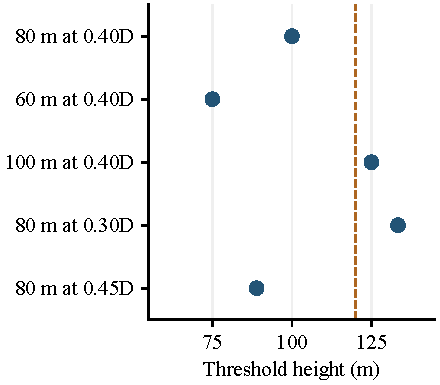
\includegraphics[width=\columnwidth]{figs/fig4_thresholds.pdf}
\caption{Relay height at which the first hop begins to clear, for the five screen cases. Thresholds above 120 m remove that altitude layer from service, while changes that stay between 60 and 120 m leave the sampled results unchanged. This is a geometric comparison, not a terrain model.}
\label{fig:thresh}
\end{figure}

%======================================================================
\section{Discussion}
%======================================================================

\subsection{What the Result Supports}

The classification tells an engineer which assumptions to revisit. A connectivity failure calls for reconsidering geometry or the link budget. More battery cannot repair that failure while the RF assumptions remain fixed. A finite result outside the size screen calls for reconsidering dwell, carrier assumptions, or the permitted physical envelope. Mathematical nonclosure calls for changing the resource relationship itself: relaxing a mass ceiling cannot create a missing fixed point.

The worked example makes these decisions concrete. At 30 minutes the carrier passes the exploratory screen and becomes a candidate for more detailed assessment. At 45 minutes the 15.15 kg result indicates excessive burden under the stated assumptions. At 60 minutes there is no consistent mass to size or cost. Treating both failed cases as a numerical convergence problem would lose the distinction between them.

The calculations also show the limits of the coupling. The payload supplies common mass, DC, and RF assumptions, but link margin does not resize the radio and altitude does not change the fixed-density hover calculation. Consequently, the case supports an architecture screening decision without solving a joint radio, trajectory, and vehicle optimization. For a systems engineering reader, its useful output is a traceable chain from the requested service to the resource or link assumption that limits it.

\subsection{Limitations}

The carrier result depends on a resized family with constant disk loading, aggregate hover efficiency, and parametric component masses. The five-point fit provides evidence for an aggregate power coefficient over those test conditions. It does not resolve scale effects, rotor interference, or environmental variation for the proposed carrier. The least-squares fit also gives greater numerical influence to high-power observations, so the DAx8 dominates it, and that point and the Endurance point were measured in the tunnel with unquantified recirculation. The spread of single-point fits, 33 to 49 minutes for the rotor-limit boundary, is a better statement of the hover-model uncertainty than the fitted value alone, and it exceeds the effect of any other estimator choice. The reference case includes no operating-condition margin beyond the laboratory calibration. The commercial hover comparisons use nominal energy and a common auxiliary-load allowance; their small discrepancies could include compensating assumptions. They should not be read as a seven-percent accuracy guarantee.

The structural relation is anchored at one conceptual mass breakdown. Its extrapolation becomes especially consequential near the closure singularity. Neither that anchor nor the power fit establishes packaging, strength, vibration response, thermal compatibility, or a realizable combination of battery energy and power. The nominal bounds remain exploratory rather than approved aircraft requirements. The repository name retains a low-cost objective, but this paper establishes no affordability result.

The link calculation tests visibility and received level. It omits interference, fading, diffraction, Fresnel clearance, scheduling, duplex operation, and throughput. Two of these simplifications are conservative. An opaque screen treats a grazing path as blocked, whereas knife-edge diffraction would impose a finite loss. However, omitting Fresnel clearance works in the other direction just above the geometric threshold. In the 10 km case, keeping 60 percent of the first Fresnel zone clear at the screen raises the 100 m threshold to about 108 m. This does not change the sampled results, since the 120 m layer still clears. The midpoint relay placement is also not optimal: the first hop binds, and moving the relay to 0.44 of the span balances the hops and raises the 25.0 km boundary to 28.3 km while still clearing the screen. Antenna patterns and interference could move the result in either direction. The screen scenarios are geometric constructions rather than surveyed terrain. Statistical air-to-ground blockage models address different questions \cite{alhourani}; none is fitted or validated here. No probability of availability follows from the number of passing grid cases.

Only stationary outbound dwell is calculated. Transit, climb, recovery energy, return traffic, carrier-command performance, and station keeping remain outside the quantitative assessment. A follow-on assessment would need matched power measurements, installed-payload characterization, a complete mission energy budget, and communications measurements for the intended service. These are evidence needs for the candidate architecture, not capabilities demonstrated by this paper.



%======================================================================
\section{Conclusions}
%======================================================================

A useful relay path and a supportable carrier are separate conditions for airborne service. This case study connects them through a declared payload and reports the limiting mechanism for each sampled mission. At the reference inputs, the midpoint relay has a 25.0 km link-margin boundary at 120 m height; 12 dB of added loss reduces it to 6.3 km. Carrier size reaches the exploratory rotor limit at 42.1 minutes, while mathematical closure ends at 52.4 minutes within the assumed model. These values include no operating-condition margin, and the scatter among the individual hover calibration points alone spans 33 to 49 minutes for the first boundary.

The 10 km example distinguishes a 4.77 kg, 30-minute pass from a 15.15 kg, 45-minute exclusion and a 60-minute nonclosure. Across 90 baseline cases, 18 pass both screens. The hover calibration and published-aircraft comparisons support a limited part of the calculation, while structural scaling and full-mission performance remain unverified. The assessment gives a systems engineer an explainable way to identify the constraint that must change before advancing a relay concept.

%======================================================================

\appendices
\section{Complete Carrier Mass Balance}
The following equations specify the component bookkeeping used in the results. Mass is in kilograms, power in watts, energy in watt-hours, area in square metres, and dwell $t$ in hours. Write $q=g/DL$, so total rotor disk area is $A=qm$, and let $k$ denote electrical propulsion power per unit mass from (4). Define
\begin{equation}
P_0=P_{\mathrm{aux}}+P_L/\eta_r,\qquad u=d_b(1-r_b).
\end{equation}
The reference values are $P_0=40.2174$ W and $u=0.72$. With thrust ratio $\tau$ and battery power margin $\mu_b$, the battery branches are
\begin{equation}
\begin{aligned}
m_E&=\alpha_E m+\beta_E,& \alpha_E&=kt/(ue),\\
\beta_E&=P_0t/(ue),&\alpha_P&=\mu_b\tau^{3/2}k/p,\\
m_P&=\alpha_Pm+\beta_P,&\beta_P&=\mu_bP_0/p.
\end{aligned}
\end{equation}
Battery mass is $m_b=\max(m_E,m_P)$. Installed nominal energy is $em_b$; on the power branch it can exceed the nominal energy required for dwell. The model applies thrust scaling to propulsion alone.

With the component coefficients in Table~\ref{tab:components}, fixed carried mass and propulsion-group mass are
\begin{equation}
\begin{aligned}
m_{\mathrm{mount}}&=m_{m0}+f_m m_L,\\
F&=m_L+m_{\mathrm{av}}+m_{\mathrm{pe}}+m_{\mathrm{mount}},\\
m_{\mathrm{prop}}&=K_pm,\quad K_p=\tau^{3/2}k/p_p+\sigma_rq.
\end{aligned}
\end{equation}
The structural allowance includes all carried mass:
\begin{equation}
m_s=m_{s0}+f_s(F+m_b+m_{\mathrm{prop}})+\sigma_sA.
\end{equation}
Substitution in $m_{\mathrm{new}}=F+m_b+m_{\mathrm{prop}}+m_s$ gives, for branch $j\in\{E,P\}$,
\begin{equation}
\begin{aligned}
a_j&=(1+f_s)(\alpha_j+K_p)+\sigma_sq,\\
b_j&=(1+f_s)(F+\beta_j)+m_{s0}.
\end{aligned}
\end{equation}
Evaluate $m_j^*=b_j/(1-a_j)$ only for $a_j<1$ and positive mass. The energy candidate is valid when $m_E(m_E^*)\geq m_P(m_E^*)$; the power candidate requires the reverse inequality at $m_P^*$. With no valid candidate, physical mass, area, power, and energy are undefined. A branch tie gives the same fixed point.

\begin{table}[!tb]
\caption{Remaining reference carrier coefficients}
\label{tab:components}
\centering\small
\begin{tabular}{@{}L{1.50in}L{1.45in}@{}}
\toprule
Quantity & Value \\
\midrule
Gravity $g$; density $\rho$ & 9.80665 m/s$^2$; 1.225 kg/m$^3$ \\
Rotor count $n$ & 4 \\
Propulsion specific power $p_p$ & 2300 W/kg \\
Rotor area mass $\sigma_r$ & 0.14 kg/m$^2$ \\
Structure fraction $f_s$ & 0.18 \\
Structure area mass $\sigma_s$ & 0.22 kg/m$^2$ \\
Avionics mass $m_{\mathrm{av}}$ & 0.40 kg \\
Power electronics $m_{\mathrm{pe}}$ & 0.28 kg \\
Mount base $m_{m0}$; fraction $f_m$ & 0.20 kg; 0.18 \\
Auxiliary power $P_{\mathrm{aux}}$ & 25 W \\
Payload regulator $\eta_r$ & 0.92 \\
Depth of discharge $d_b$ & 0.90 \\
Reserve fraction $r_b$ & 0.20 \\
Thrust ratio $\tau$; margin $\mu_b$ & 1.75; 1.15 \\
\bottomrule
\end{tabular}
\end{table}

For reproduction, the reference effective $FM$ is 0.620274, structure intercept is 0.163173 kg, and specific energy is 192.117 Wh/kg. Other nominal values appear in Table~\ref{tab:inputs}. These numerical precisions identify inputs, not measurement accuracy. The 1.5 m span proxy equals twice rotor diameter and repeats the 0.75 m rotor screen. The full input catalog supplies the simultaneous favorable and adverse parameter sets; those corners are not used for the primary 90-case counts.

\section*{Data Availability}
%======================================================================

The computational baseline, declared inputs, calibration data, 1,890 case records, tests, and independent checker are identified at \url{https://github.com/noahstephenson/low-cost-relay-uas} (branch codex/carrier-calibration-v1; computational baseline at commit 4f9e2cd). The manuscript source is in the repository's submission directory under a Creative Commons Attribution 4.0 license.

\section*{Acknowledgments}

The views expressed in this paper are those of the author. They do not reflect the official policy or position of the United States Military Academy, the Department of the Army, the Department of Defense, or the U.S. Government.

%======================================================================
\begin{thebibliography}{99}
\small
\setlength{\itemsep}{1pt}

\bibitem{zengmag} Y. Zeng, R. Zhang, and T. J. Lim, ``Wireless communications with unmanned aerial vehicles: Opportunities and challenges,'' \emph{IEEE Commun. Mag.}, vol. 54, no. 5, pp. 36-42, May 2016, doi: 10.1109/MCOM.2016.7470933.

\bibitem{tutorial} M. Mozaffari, W. Saad, M. Bennis, Y.-H. Nam, and M. Debbah, ``A tutorial on UAVs for wireless networks: Applications, challenges, and open problems,'' \emph{IEEE Commun. Surveys Tuts.}, vol. 21, no. 3, pp. 2334-2360, 2019, doi: 10.1109/COMST.2019.2902862.

\bibitem{zengrelay} Y. Zeng, R. Zhang, and T. J. Lim, ``Throughput maximization for UAV-enabled mobile relaying systems,'' \emph{IEEE Trans. Commun.}, vol. 64, no. 12, pp. 4983-4996, Dec. 2016, doi: 10.1109/TCOMM.2016.2611512.

\bibitem{zengenergy} Y. Zeng, J. Xu, and R. Zhang, ``Energy minimization for wireless communication with rotary-wing UAV,'' \emph{IEEE Trans. Wireless Commun.}, vol. 18, no. 4, pp. 2329-2345, Apr. 2019, doi: 10.1109/TWC.2019.2902559.

\bibitem{yan} H. Yan, S.-H. Yang, Y. Chen, and S. A. Fahmy, ``Optimum battery weight for maximizing available energy in UAV-enabled wireless communications,'' \emph{IEEE Wireless Commun. Lett.}, vol. 10, no. 7, pp. 1410-1413, Jul. 2021, doi: 10.1109/LWC.2021.3069078.

\bibitem{rodrigues} H. Rodrigues, A. Coelho, M. Ricardo, and R. Campos, ``Energy-aware relay positioning in flying networks,'' \emph{Int. J. Commun. Syst.}, vol. 35, no. 13, Art. no. e5233, 2022, doi: 10.1002/dac.5233.

\bibitem{russell2018} C. R. Russell, C. R. Theodore, and M. K. Sekula, ``Incorporating test data for small UAS at the conceptual design level,'' in \emph{Proc. AHS Int. Tech. Meeting Aeromechanics Design Transformative Vertical Flight}, San Francisco, CA, USA, Jan. 2018. [Online]. Available: \url{https://rotorcraft.arc.nasa.gov/Publications/files/Russell_2018_TechMx.pdf}

\bibitem{bershadsky} D. Bershadsky, S. Haviland, and E. N. Johnson, ``Electric multirotor UAV propulsion system sizing for performance prediction and design optimization,'' in \emph{Proc. 57th AIAA/ASCE/AHS/ASC Structures, Structural Dynamics, and Materials Conf.}, San Diego, CA, USA, Jan. 2016, doi: 10.2514/6.2016-0581.

\bibitem{nasatm} C. Russell, G. Willink, C. Theodore, J. Jung, and B. Glasner, ``Wind tunnel and hover performance test results for multicopter UAS vehicles,'' NASA, Moffett Field, CA, USA, Rep. NASA/TM-2018-219758, Feb. 2018. [Online]. Available: \url{https://rotorcraft.arc.nasa.gov/Publications/files/Russell_1180_Final_TM_022218.pdf}

\bibitem{djim30} DJI, ``Matrice 30 series specifications,'' product page. Accessed: Sep. 11, 2026. [Online]. Available: \url{https://enterprise.dji.com/matrice-30/specs}

\bibitem{doodle} Doodle Labs, ``OEM Mesh Rider Radio: Hardware and RF specifications,'' product page. Accessed: Sep. 11, 2026. [Online]. Available: \url{https://doodlelabs.com/product/oem/}

\bibitem{itu525} \emph{Calculation of Free-Space Attenuation}, ITU-R Recommendation P.525-5, Nov. 2024. [Online]. Available: \url{https://www.itu.int/rec/R-REC-P.525-5-202411-I/en}

\bibitem{friis} H. T. Friis, ``A note on a simple transmission formula,'' \emph{Proc. IRE}, vol. 34, no. 5, pp. 254-256, May 1946, doi: 10.1109/JRPROC.1946.234568.

\bibitem{leishman} J. G. Leishman, \emph{Principles of Helicopter Aerodynamics}, 2nd ed. Cambridge, U.K.: Cambridge Univ. Press, 2006.

\bibitem{ndarc} W. Johnson, ``NDARC: NASA Design and Analysis of Rotorcraft, Theory, Appendix 3,'' NASA, Moffett Field, CA, USA, Rep. NASA/TP-2009-215402, Release 1.7, Dec. 2012. [Online]. Available: \url{https://rotorcraft.arc.nasa.gov/Publications/files/NASA\%20TP-2009-215402-app3.pdf}

\bibitem{djim4} DJI, ``Matrice 4 series specifications,'' product page. Accessed: Sep. 11, 2026. [Online]. Available: \url{https://enterprise.dji.com/matrice-4-series/specs}

\bibitem{djimavic} DJI, ``Mavic 3M specifications,'' product page. Accessed: Sep. 11, 2026. [Online]. Available: \url{https://enterprise.dji.com/mavic-3-m/specs}

\bibitem{russell2016} C. Russell, J. Jung, G. Willink, and B. Glasner, ``Wind tunnel and hover performance test results for multicopter UAS vehicles,'' in \emph{Proc. AHS 72nd Annual Forum}, West Palm Beach, FL, USA, May 2016. [Online]. Available: \url{https://ntrs.nasa.gov/citations/20160007399}

\bibitem{alhourani} A. Al-Hourani, S. Kandeepan, and S. Lardner, ``Optimal LAP altitude for maximum coverage,'' \emph{IEEE Wireless Commun. Lett.}, vol. 3, no. 6, pp. 569-572, Dec. 2014, doi: 10.1109/LWC.2014.2342736.

\end{thebibliography}

\section*{Biography}

\noindent\textbf{Noah Stephenson} is a cadet in the Class of 2027 at the United States Military Academy at West Point, where he majors in Systems Engineering with a track in Cyber Security Engineering. His interests include defense technology, systems architecture, and translating operational problems into system designs. His current work applies model-based systems engineering to small uncrewed aircraft and communications systems.

\end{document}

